\documentclass{article}
\usepackage[english]{babel}
\usepackage[utf8]{inputenc}
\usepackage{fancyhdr}
\usepackage{geometry}
\usepackage{enumitem}
\usepackage{amsmath}
\usepackage{graphicx}
\usepackage{tcolorbox}
\usepackage{amssymb}
\usepackage[thinc]{esdiff}
\usepackage{float}

\geometry{letterpaper, portrait, margin=1in}
\graphicspath{ {images/} }
\pagestyle{fancy}
\fancyhf{}
\lhead{Keerthik Muruganandam}
\rhead{Written Work 13}

\begin{document}

\begin{enumerate}[label=\textbf{(13.\arabic*)}]

\item If $a$ and $b$ are positive numbers, find the maximum value of $f(x)=x^a(1-x)^b$, $0\le x\le 1$.

To find critical points, we will take the derivative of the function $f(x)=x^a(1-x)^b$, and solve for 0.
\begin{align*}
f^\prime(x)&=\diff{ }{x}\left(x^a(1-x)^b\right) \\
&=\diff{ }{x}\left(x^a\right)(1-x)^b+\diff{ }{x}\left((1-x)^b\right)x^a \\
&=(ax^{a-1})(1-x)^b+b(1-x)^{b-1}\diff{ }{x}(1-x)x^a \\
&=-x^ab(1-x)^{b-1}+a(x-1)^bx^{a-1} \\
&=x^{a-1}(1-x)^{b-1}[(1-x)a-bx] \\
&=x^{a-1}(1-x)^{b-1}[a-x(a+b)] \\
\end{align*}
Now to find the critical points, we must solve for $f^\prime=0$.
\[x^{a-1}(1-x)^{b-1}[a-x(a+b)]=0\]
From here we can see that x must either equal 0, 1 , or $\dfrac{a}{a+b}$. Because we are trying to find the maximum on the interval [0,1], the critical points must be on the open interval (0,1). Thus, we can eliminate $x=0$ and $x=1$ from the pool of possible critical points, leaving $x=\dfrac{a}{a+b}$ as the only possible critical point on the interval.\\
Now that we have our critical point, we can just solve $f(\dfrac{a}{a+b})$ to find the possible maximum of the function in the interval $0\le x\le 1$.
\begin{align*}
f\left(\frac{a}{a+b}\right)&={\left(\frac{a}{a+b}\right)}^a{\left(1-\frac{a}{a+b}\right)}^b \\
&={\left(\frac{a}{a+b}\right)}^a{\left(\frac{b}{a+b}\right)}^b \\
&= \frac{a^a}{{\left(a+b\right)}^a}\cdot\frac{b^b}{{\left(a+b\right)}^b} \\
&=\frac{a^ab^b}{{\left(a+b\right)}^{a+b}}
\end{align*}
To determine whether $\dfrac{a}{a+b}$ is a maximum, we must check if $f(0) \text{ and } f(1)$ are greater than $f\left(\dfrac{a}{a+b}\right)$.
\begin{align*}
f(0)&=0^a(1-0)^b \\
&=0\cdot1^b \\
&=0 \\
f(1)&=1^a(1-1)^b \\
&=1^a\cdot0
&=0
\end{align*}
Now we know that $\dfrac{a}{a+b}$ is the maximum point because $a \text{ and } b$ are positive numbers and thus are greater than 0.
\begin{tcolorbox}[colback=white]
The maximum value of  $f(x)=x^a(1-x)^b$, $0\le x\le 1$ is $\dfrac{a^ab^b}{{\left(a+b\right)}^{a+b}}$
\centering
\end{tcolorbox}

\par
Next Page.$ \rightarrow$
\newpage
\item Sketch a function $f$ that satifisfies all of the following conditions (simultaneously):
\begin{enumerate}[label=(\alph*)]
\item $f^\prime(x) > 0 \text{ if } |x| < 2, f^\prime(x) < 0 \text{ if }|x| > 2$
\item $x=2$ is a critical number
\item $\lim_{x \to \infty} {f(x)} = 1$
\item $f(-x)=-f(x)$
\item $f^{\prime\prime}(x) < 0 \text{ if } 0<x<3\text{, }f^{\prime\prime}(x)>0\text{ if }x>3$ \\
\newline
\end{enumerate}
Now we will interpret what each of the conditions mean to help us sketch our graph. \\
The condition $a$) means that the function is increasing from (-2,2) and decreasing everywhere else. When we take into account condition $(b)$, 2 is a maximum and then it goes down to the line $y=$ because there is a horizontal asymptote there from condition $(c)$. The function $f$ will also be reflected over the origin because of $(d)$, so everything that we said before now also holds true for the 3rd quadrant. And finally, $(e)$ means that the function will be concave down for (0,3) and concave up elsewhere. \\ This is a graph of the function that satfisfies all of those conditions: \\
\par
\begin{figure}[H]
\centering
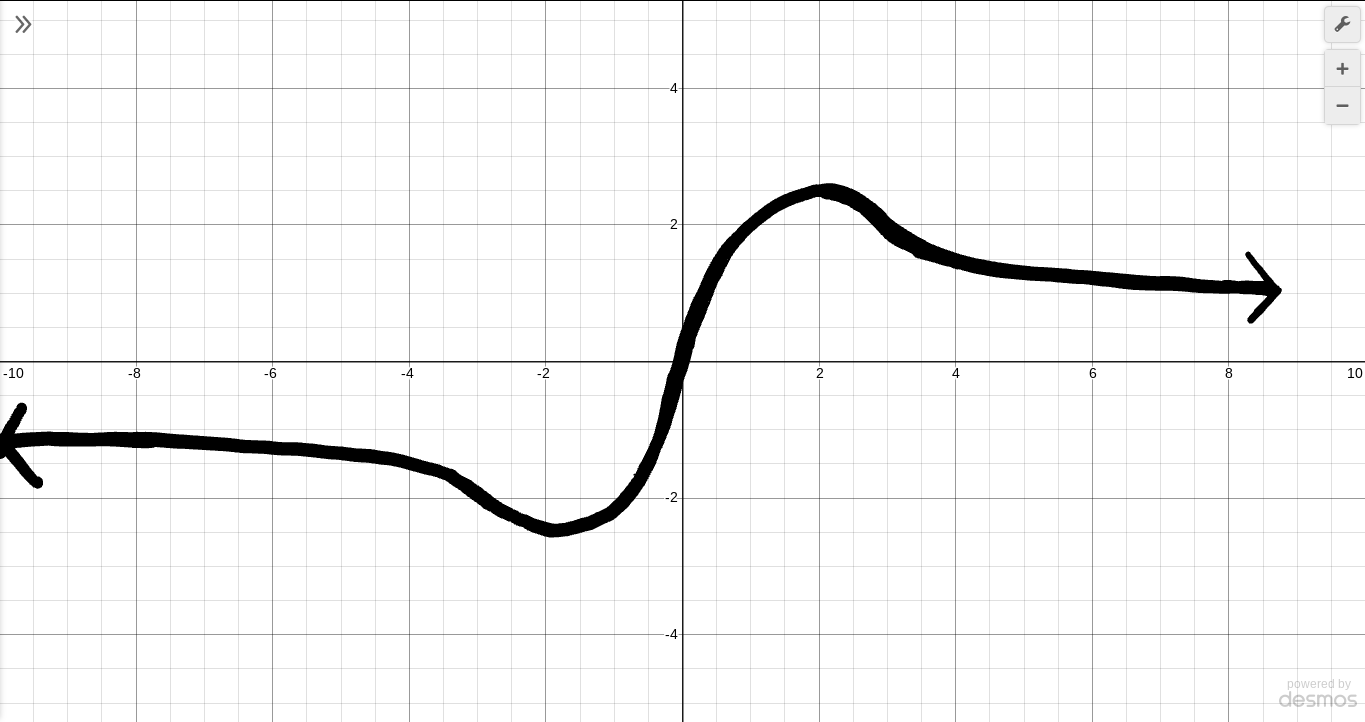
\includegraphics[scale=.2]{ink}
\end{figure}

We can see that both local and global maximums are the same, and there is only one local maximum. The local and global maximum is $(2,2.5)$ and the local and global minimum is $(-2,-2.5)$.

\item For the function $f(x)=\dfrac{x^2}{(x-4)^2}$
\begin{enumerate}[label=\alph*]
\item Find the vertical and horizontal asymptotes
\item Find the open intervals of increase and decrease
\item Find local maximums and minimums
\item Find open intervals of concavity and inflection points
\item Use the information from the parts above to sketch $f$.
\end{enumerate}\
\begin{enumerate}[label=(\alph*)]
\item HA:
\begin{align*}
\lim_{x \to \infty} {\frac{x^2}{{(x-4)}^2}}&= {\left(\lim_{x\to\infty} {\frac{x}{x-4}}\right)}^2 \\
&= {\left(\lim_{x\to\infty} {\frac{1}{1-\frac{4}{x}}}\right)}^2 \\
&= {\left(\frac{1}{1}\right)}^2 \\
&= 1
\end{align*}
VA:
Vertical asymptote is at $x=4$ because the denominator of $f$ is undefined at 4.
\item $f^\prime(x)=\frac{-8x}{(x-4)^3}$. $f(x)$ is negative when $-\infty<x<0$ and $4<x<\infty$. $x$ is increasing on the intervals $(-\infty,0)\text{U}(4,\infty)$. $x$ is increasing on the interval $(0,4)$.
\item $f^\prime(x)=\frac{-8x}{(x-4)^3}$. $f^\prime(x)$ is equal to 0 at $x=0$. $f(x)$ has a global and local minimum at $(0,0)$ and no maximum.
\item $f^{\prime\prime}(x)=\frac{16(x+2)}{(x-4)^{4}}$. Intervals are: Concave down: ($-\infty$,-2) and Concave up: (-2,$\infty$). Thus the inflection point is $-2$.
\item My figure of the equation is:
 \begin{figure}[H]
\centering
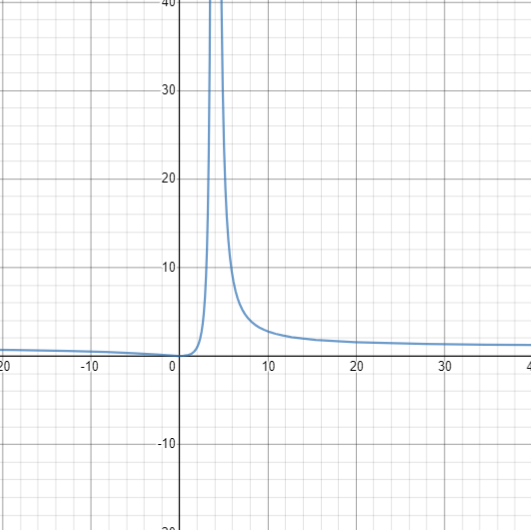
\includegraphics[scale=.5]{graph8}
\end{figure}
\end{enumerate}

\newpage

\item \textbf{Professional Problem:} A cubic function is a polynomial of degree 3. It has the form $f(x)=ax^3+bx^2+cx+d$, where $a$, $b$, $c$, and $d$ are real numbers and $a\neq0$.
\begin{enumerate}[label=(\alph*)]
\item Prove that a cubic function can have two, one, or no critical numbers by providing explicit examples. Sketch your examples.
\item How many local extrema can a cubic function have? Provide explicit examples that exhibit each possibility; sketch your examples. Prove that you have found all of the possibilities.
\end{enumerate}
\begin{enumerate}[label=(\alph*)]
\item For two solutions, we can take the derivative
\begin{align*}
f^\prime(x)&=3x^2+4x+1 \\
&=(3x+1)(x+1)
\end{align*}
 For the function with one solution we can take the derivative
\[f^\prime(x)=(x+1)^2\]
For the function with no solutions, we take the derivative
\[f^\prime(x)=3x^2+2x^2+1\]
\begin{figure}[H]
\centering
\begin{minipage}{.3\textwidth}
  \centering
  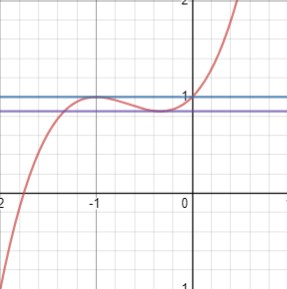
\includegraphics[width=.4\linewidth]{graph5}
  \caption{2 extrema}
  \label{fig:test1}
\end{minipage}%
\begin{minipage}{.3\textwidth}
  \centering
  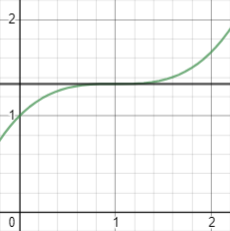
\includegraphics[width=.4\linewidth]{graph6}
  \caption{1 extrema}
  \label{fig:test2}
\end{minipage}
\begin{minipage}{.3\textwidth}
  \centering
  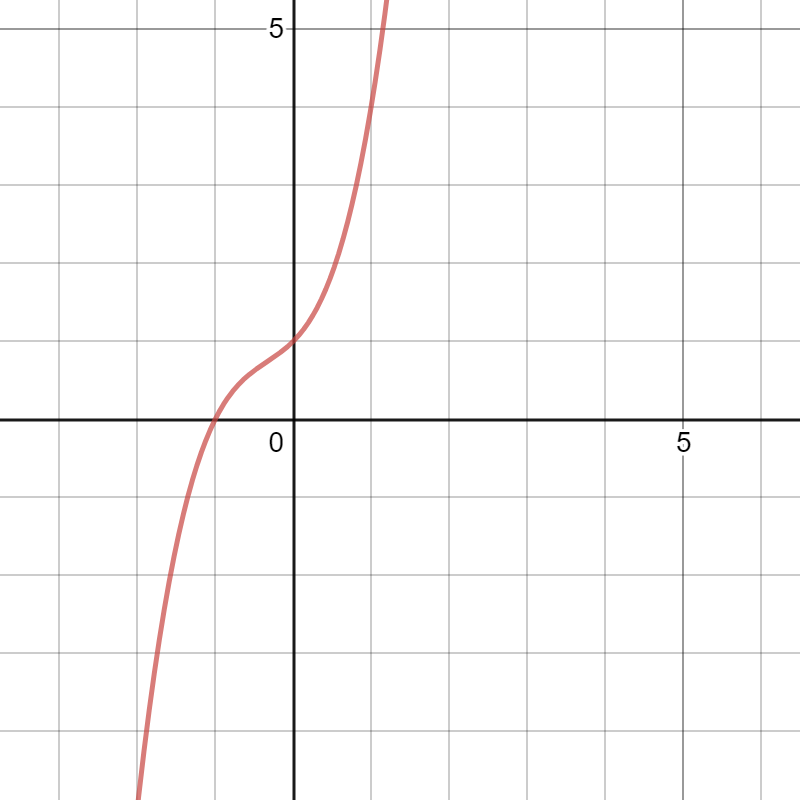
\includegraphics[width=.4\linewidth]{graph7}
  \caption{No extrema}
  \label{fig:test3}
\end{minipage}
\end{figure}
\item A cubic function can have 0, 1, or 2 extrema. My examples are:
\begin{figure}[H]
\centering
\begin{minipage}{.3\textwidth}
  \centering
  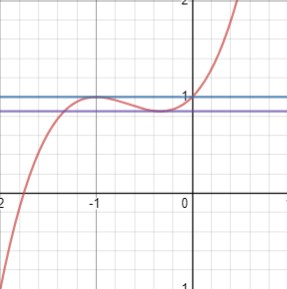
\includegraphics[width=.4\linewidth]{graph5}
  \caption{2 extrema}
  \label{fig:test1}
\end{minipage}%
\begin{minipage}{.3\textwidth}
  \centering
  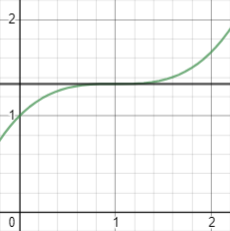
\includegraphics[width=.4\linewidth]{graph6}
  \caption{1 extrema}
  \label{fig:test2}
\end{minipage}
\begin{minipage}{.3\textwidth}
  \centering
  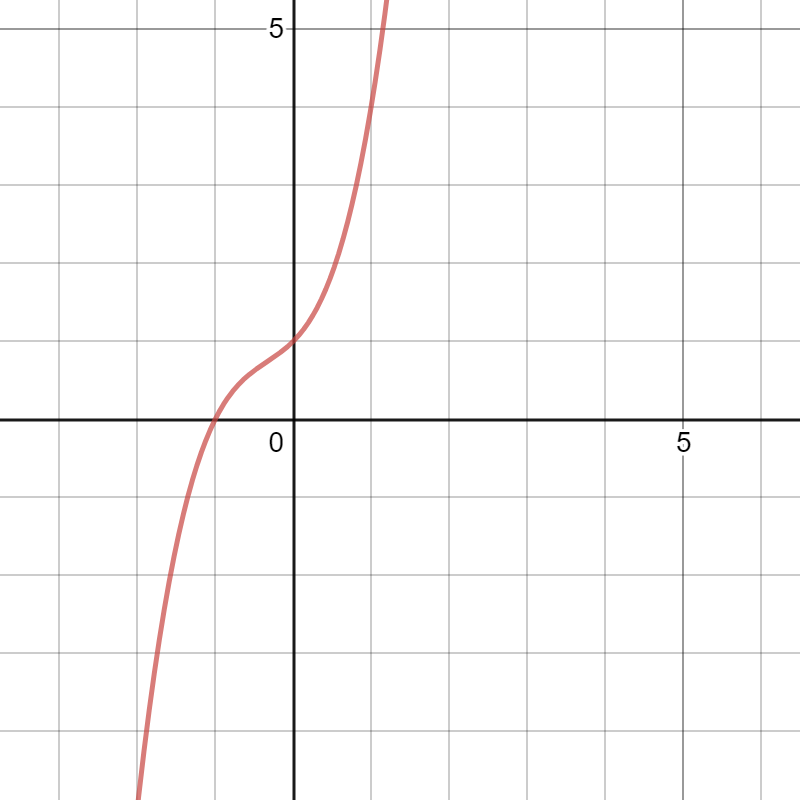
\includegraphics[width=.4\linewidth]{graph7}
  \caption{No extrema}
  \label{fig:test3}
\end{minipage}
\end{figure}
\end{enumerate}
A function's extrema are critical points, or points whose tangent lines have a slope of 0. The critical points then, are points for which the derivative of the function solves for 0. The derivative of a cubic function
\[f(x)=ax^3+bx^2+cx+d\text{,}\]
is
\[f^\prime(x)=3ax^2+2bx+c\]
From here we can see that the derivative of a cubic polynomial is a quadratic polynomial. Now, from the discriminant, we can tell that a quadratic, at most, can have 2 solutions and at least, 0. Therefore, a cubic function can have either 0, 1, or 2 extrema.

\end{enumerate}


\end{document}